
% ============================================================
%  RMC — Reconfigurable DDR5 Memory Controller
%  Architecture & Design Decisions — v1.9.8
%  Beamer presentation
%  Style/preamble reused verbatim from memory_ctl/rocky.tex
%  Compile:  pdflatex -shell-escape RMC_Architecture_Ideas_v1.9.8.tex
%            (run twice for cross-refs)
% ============================================================
\documentclass[aspectratio=169,10pt]{beamer}

% ── Packages ────────────────────────────────────────────────────────────────
\usepackage{tikz}
\usetikzlibrary{arrows.meta, fit, backgrounds, calc, positioning, matrix}
\usepackage{xcolor}
\usepackage[T1]{fontenc}
\usepackage{lmodern}
\usepackage{amsmath}
\usepackage{booktabs}
\usepackage{colortbl}
\usepackage{array}
\usepackage{microtype}
\usepackage{hyperref}
\usepackage{graphicx}

% ── Palette ─────────────────────────────────────────────────────────────────
\definecolor{Navy}   {HTML}{0D1B2A}
\definecolor{Teal}   {HTML}{1A6060}
\definecolor{TealF}  {HTML}{D4EEEE}
\definecolor{Blue}   {HTML}{1A3A7A}
\definecolor{BlueF}  {HTML}{DDE3F5}
\definecolor{Amber}  {HTML}{7A4010}
\definecolor{AmberF} {HTML}{FAE8D4}
\definecolor{Purp}   {HTML}{534AB7}
\definecolor{PurpF}  {HTML}{EEEDFE}
\definecolor{Green}  {HTML}{3B6D11}
\definecolor{GreenF} {HTML}{EAF3DE}
\definecolor{MGray}  {HTML}{5F5E5A}
\definecolor{LGray}  {HTML}{E8EBF0}
\definecolor{BypassR}{HTML}{993C1D}

% ── Beamer theme ────────────────────────────────────────────────────────────
\usetheme{default}
\usecolortheme{default}
\setbeamertemplate{navigation symbols}{}
\setbeamertemplate{frametitle}{%
  \begin{beamercolorbox}[wd=\paperwidth,ht=0.72cm,dp=0pt,leftskip=0.35cm]{frametitle}%
    \vbox to 0.72cm{\vfil
      \usebeamerfont{frametitle}\insertframetitle
      \ifx\insertframesubtitle\@empty\else
        \hfill{\footnotesize\color{cyan!60!white}\insertframesubtitle}%
      \fi
    \hspace*{0.35cm}\vfil}%
  \end{beamercolorbox}%
}
\setbeamercolor{frametitle}{bg=Navy, fg=white}
\setbeamerfont{frametitle}{size=\large,series=\bfseries}
\setbeamercolor{background canvas}{bg=LGray!30!white}
\setbeamercolor{normal text}{fg=Navy}
\setbeamertemplate{footline}{%
  \hfill{\tiny\color{MGray}\insertframenumber/\inserttotalframenumber\hspace*{4pt}}%
  \vspace*{3pt}%
}

% ── TikZ block styles ────────────────────────────────────────────────────────
\tikzset{
  blk/.style args={#1/#2}{
    rectangle, rounded corners=4pt,
    draw=#1, fill=#2, text=#1,
    font=\scriptsize\bfseries, align=center,
    inner sep=5pt, minimum width=2.0cm, minimum height=0.75cm,
    line width=0.8pt,
  },
  sblk/.style args={#1/#2}{
    rectangle, rounded corners=3pt,
    draw=#1, fill=#2, text=#1,
    font=\tiny\bfseries, align=center,
    inner sep=3pt, minimum width=1.6cm, minimum height=0.6cm,
    line width=0.7pt,
  },
  rgn/.style args={#1}{
    draw=#1, fill=#1!6, rounded corners=6pt,
    dashed, line width=0.9pt,
  },
  arr/.style args={#1}{
    -{Stealth[length=4pt,width=3pt]},
    line width=0.8pt, color=#1,
  },
  lbl/.style={
    font=\tiny\itshape, text=MGray,
    fill=white, inner sep=1pt,
  },
}

% ── Info card helper ─────────────────────────────────────────────────────────
\newcommand{\infocard}[3]{%
  \begin{tikzpicture}
    \node[rectangle, rounded corners=4pt,
          draw=#1, fill=#2, text=Navy,
          inner sep=7pt, line width=0.9pt,
          text width=\linewidth-14pt-2\pgflinewidth] {#3};
  \end{tikzpicture}%
}

% ============================================================
\begin{document}

% ── Slide 1: Title ───────────────────────────────────────────────────────────
\setbeamercolor{background canvas}{bg=Navy}
\begin{frame}[plain]
  \vspace*{0.6cm}
  \begin{center}
    {\huge\bfseries\color{white}RMC — Reconfigurable DDR5 Memory Controller}\\[6pt]
    {\large\color{cyan!70!white}Architecture \& Design Decisions — v1.9.8}\\[4pt]
    {\small\color{blue!40!white}JESD79-5 \quad|\quad AXI4 Host Interface \quad|\quad DFI 5.2 PHY}
  \end{center}
  \vspace*{0.4cm}
  {\color{Navy!40!white}\rule{\linewidth}{0.4pt}}
  \vspace*{0.3cm}
  \begin{center}
    {\scriptsize\color{blue!40!white}%
    4GB single-channel single-rank anchor config $\;\to\;$ 46b address, 8ch, 8rank, 64Gb$\times$3DS-8H = 64TB ceiling\\[3pt]
    RTL style: SystemVerilog, fully parameterized, zero hardcoded widths\\[3pt]
    Architecture status: complete \quad$\vert$\quad RTL status: skeleton not started}
  \end{center}
\end{frame}
\setbeamercolor{background canvas}{bg=LGray!30!white}

% ── Slide 2: Scope ───────────────────────────────────────────────────────────
\begin{frame}{Project Identity \& Scope}
              {What RMC is, and deliberately is not}
  \begin{columns}[T,totalwidth=\linewidth]
    \begin{column}{0.49\linewidth}
      \infocard{Blue}{BlueF}{%
        {\small\bfseries\color{Blue}In Scope}\\[3pt]
        \scriptsize
        \textbullet\ DDR5 command pipeline: split, translate, buffer, schedule\\[2pt]
        \textbullet\ CAM-searched write/read buffers + RAW hazard bypass\\[2pt]
        \textbullet\ 5-stage bank-aware SJF command scheduler\\[2pt]
        \textbullet\ Per-bank / per-rank / global JEDEC timing state\\[2pt]
        \textbullet\ 6 sub-FSM maintenance engine (init, refresh, ZQ, RFM,\\
        \phantom{\textbullet\ }power mgmt, thermal poll)\\[2pt]
        \textbullet\ Address hierarchy: Ch $\to$ Subch $\to$ Rank $\to$ BG $\to$ Bank $\to$ Row $\to$ Col
      }
    \end{column}
    \begin{column}{0.49\linewidth}
      \infocard{Amber}{AmberF}{%
        {\small\bfseries\color{Amber}Out of Scope}\\[3pt]
        \scriptsize
        \textbullet\ DDR PHY — DFI 5.2 is the fixed contract boundary\\[2pt]
        \textbullet\ AXI masters / interconnect upstream of the host port\\[2pt]
        \textbullet\ AXI WRAP/FIXED bursts, narrow/unaligned transfers\\[2pt]
        \textbullet\ Exclusive access, QoS ordering\\[2pt]
        \textbullet\ Runtime DIMM discovery (OQ-20, closed out of scope)
      }

      \vspace{6pt}
      \infocard{Purp}{PurpF}{%
        {\small\bfseries\color{Purp}Baseline Anchor Config}\\[3pt]
        \scriptsize
        4GB \textbullet\ single channel \textbullet\ single rank\\
        32b address \textbullet\ scales to 46b / 8ch / 8rank / 3DS-8H
      }
    \end{column}
  \end{columns}
\end{frame}

% ── Slide 3: Foundational Locks I ────────────────────────────────────────────
\begin{frame}{Foundational Locks (I)}
              {Decisions that shape everything downstream}
  \infocard{Teal}{TealF}{%
    {\small\bfseries\color{Teal}BL16-Only Burst Model}\\[2pt]
    \scriptsize A 64B AXI-aligned INCR burst = exactly one BL16 burst on a 32b DDR5
    subchannel. One AXI beat-group $\equiv$ one DRAM burst, always — no fragment
    bookkeeping anywhere downstream.
  }
  \vspace{5pt}
  \infocard{Blue}{BlueF}{%
    {\small\bfseries\color{Blue}Deliberately Narrow AXI Feature Set}\\[2pt]
    \scriptsize INCR only, 64-bit data, multiple outstanding IDs — but no
    narrow/unaligned, no exclusive access, no QoS. Every cut feature added
    verification surface without adding value for a DRAM controller.
  }
  \vspace{5pt}
  \infocard{Amber}{AmberF}{%
    {\small\bfseries\color{Amber}Exactly One Clock-Domain Crossing}\\[2pt]
    \scriptsize CIF = AXI clock. MC core = MC clock. The \emph{only} meeting point
    is one async-FIFO pair (req + resp). 100\% of CDC verification burden
    concentrated into one well-understood primitive.
  }
\end{frame}

% ── Slide 4: Foundational Locks II ───────────────────────────────────────────
\begin{frame}{Foundational Locks (II)}
              {Removing $\sim$200 decrementers}
  \infocard{Purp}{PurpF}{%
    {\small\bfseries\color{Purp}Valid-Credit Everywhere Inside MC Core}\\[2pt]
    \scriptsize No combinational \texttt{ready} anywhere intra-MC — that's exactly
    what breaks timing closure at frequency. Every path uses registered credit
    counters instead. AXI ports are the one exception (spec-mandated valid-ready).
  }
  \vspace{5pt}
  \infocard{Green}{GreenF}{%
    {\small\bfseries\color{Green}Absolute Deadlines, Not Countdown Counters}\\[2pt]
    \scriptsize \texttt{next\_legal = gc + delay} stored once; every cycle:
    \texttt{eligible = (gc - next\_legal)[MSB]==0}. Same trick as TCP sequence-number
    wraparound. Collapses $\sim$200 decrementers into $\sim$100 static comparators
    against one shared free-running counter.
  }
  \vspace{5pt}
  \infocard{BypassR}{LGray}{%
    {\small\bfseries\color{BypassR}Registered can\_* Flags, Off the Critical Path}\\[2pt]
    \scriptsize Even the comparison above is computed in the background every
    cycle and stored as a plain bit. Scheduler Stage 2 \emph{only reads} these
    flags — zero subtractors in the scheduling critical path.
  }
\end{frame}

% ── Slide 5: High-Level Architecture ─────────────────────────────────────────
\begin{frame}{High-Level Architecture}
              {Seven domains, one direction of flow}
  \vspace*{-0.1cm}
  \begin{center}
  \scalebox{0.60}{%
  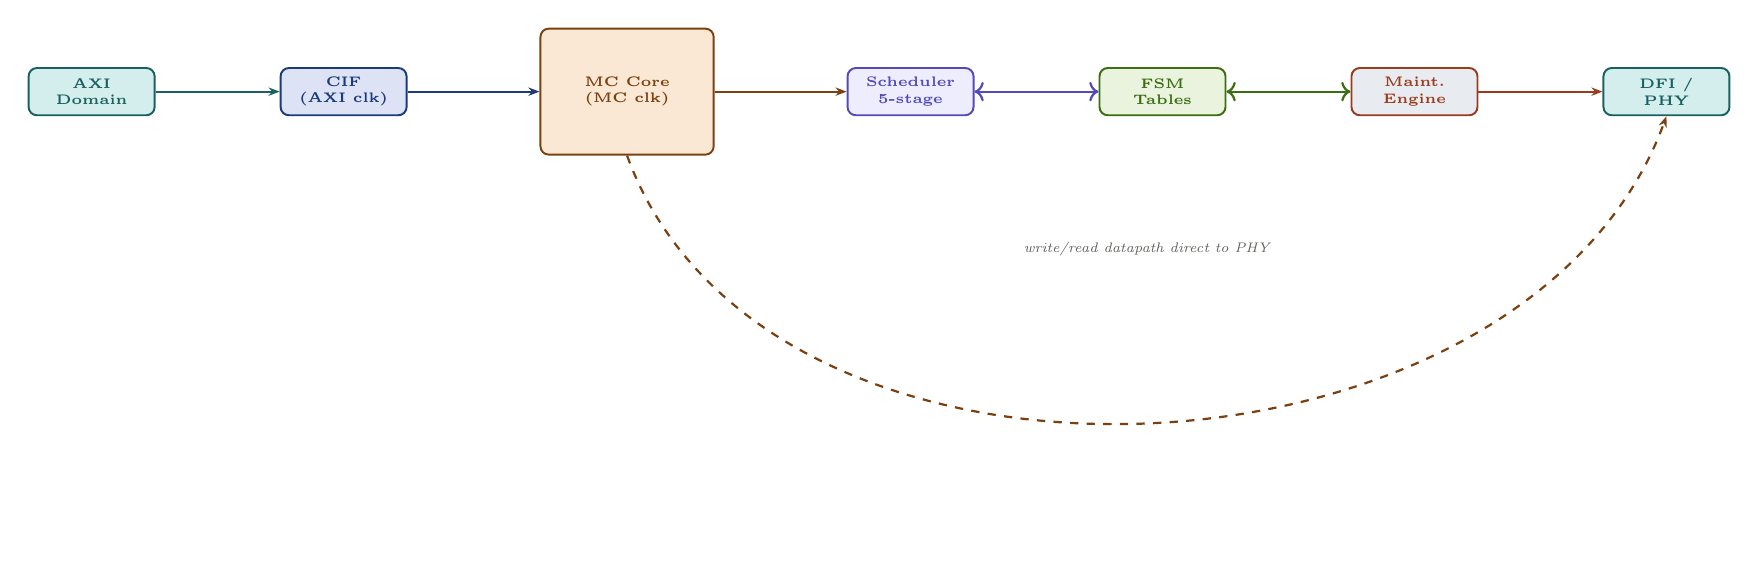
\begin{tikzpicture}[x=1cm,y=1cm]
    \node[sblk=Teal/TealF]  (axi) at (0,0)     {AXI\\Domain};
    \node[sblk=Blue/BlueF]  (cif) at (3.2,0)   {CIF\\(AXI clk)};
    \node[sblk=Amber/AmberF,minimum width=2.2cm,minimum height=1.6cm]
                            (mcc) at (6.8,0)   {MC Core\\(MC clk)};
    \node[sblk=Purp/PurpF]  (sch) at (10.4,0)  {Scheduler\\5-stage};
    \node[sblk=Green/GreenF](fsm) at (13.6,0)  {FSM\\Tables};
    \node[sblk=BypassR/LGray](me) at (16.8,0)  {Maint.\\Engine};
    \node[sblk=Teal/TealF]  (dfi) at (20.0,0)  {DFI /\\PHY};

    \draw[arr=Teal]    (axi)--(cif);
    \draw[arr=Blue]    (cif)--(mcc);
    \draw[arr=Amber]   (mcc)--(sch);
    \draw[arr=Purp,<->](sch)--(fsm);
    \draw[arr=Green,<->](fsm)--(me);
    \draw[arr=BypassR] (me)--(dfi);
    \draw[arr=Amber,dashed] (mcc.south) to[out=-70,in=-110] (dfi.south);
    \node[lbl] at (13.4,-2.0) {write/read datapath direct to PHY};

  \end{tikzpicture}}
  \end{center}
  \vspace{6pt}
  \infocard{MGray}{LGray}{%
    \scriptsize \textbf{Reading the flow:} host requests enter left, get split/hashed/
    reordered in CIF, cross the single CDC boundary into MC Core (buffers, TCAM search,
    RAW bypass), get arbitrated by the Scheduler against state held in the FSM Tables,
    with the Maintenance Engine injecting refresh/ZQ/RFM/power/thermal events and owning
    the DFI mux until handoff, out to DFI/PHY and the DRAM itself.
  }
\end{frame}

% ── Slide 6: CIF Walkthrough ──────────────────────────────────────────────────
\begin{frame}{CIF — Client Interface}
              {AXI termination $\rightarrow$ normalized, CDC-ready command stream}
  \begin{center}
  \scalebox{0.72}{%
  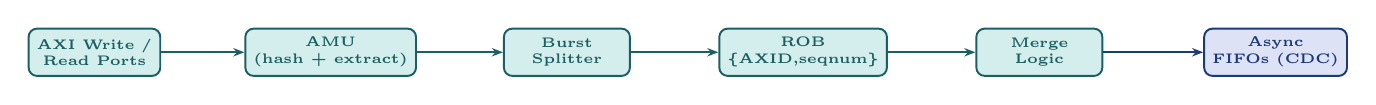
\begin{tikzpicture}[x=1cm,y=1cm]
    \node[sblk=Teal/TealF] (wp) at (0,0)    {AXI Write /\\Read Ports};
    \node[sblk=Teal/TealF] (amu) at (3,0)   {AMU\\(hash + extract)};
    \node[sblk=Teal/TealF] (bs) at (6,0)    {Burst\\Splitter};
    \node[sblk=Teal/TealF] (rob) at (9,0)   {ROB\\\{AXID,seqnum\}};
    \node[sblk=Teal/TealF] (mrg) at (12,0)  {Merge\\Logic};
    \node[sblk=Blue/BlueF] (fifo) at (15,0) {Async\\FIFOs (CDC)};
    \draw[arr=Teal] (wp)--(amu); \draw[arr=Teal] (amu)--(bs);
    \draw[arr=Teal] (bs)--(rob); \draw[arr=Teal] (rob)--(mrg);
    \draw[arr=Blue] (mrg)--(fifo);
  \end{tikzpicture}}
  \end{center}
  \vspace{4pt}
  \infocard{Teal}{TealF}{%
    {\small\bfseries\color{Teal}AMU replaces the plain Address Translator}\\[2pt]
    \scriptsize Optional per-field XOR hash (\texttt{hashed = raw XOR (raw >> shift)})
    before extracting ch/rank/bg/bank/row/col. Rank + channel hashed and pushed to
    address MSBs (spread traffic); bg/bank/row/col left un-hashed (preserve row-hit
    locality — what read latency actually depends on). Split-field extraction
    supports arbitrary channel-interleave granularity, CSR-configurable at runtime.
  }
\end{frame}

% ── Slide 7: MC Core Buffering + TCAM Split ──────────────────────────────────
\begin{frame}{MC Core — Buffering \& the TCAM Split}
              {Two different search jobs, two different CAM shapes}
  \begin{columns}[T,totalwidth=\linewidth]
    \begin{column}{0.49\linewidth}
      \infocard{Amber}{AmberF}{%
        {\small\bfseries\color{Amber}WR\_TCAM}\\[2pt]
        \scriptsize \textbf{Full} address match: \texttt{\{bg,bank,row,col\}}\\
        Job: exact-match RAW hazard detection — does an\\incoming read collide with a
        pending write?\\[2pt]
        24{,}576T baseline
      }
    \end{column}
    \begin{column}{0.49\linewidth}
      \infocard{Blue}{BlueF}{%
        {\small\bfseries\color{Blue}RD\_TCAM}\\[2pt]
        \scriptsize \textbf{Ternary} match: \texttt{\{bg,bank\}} only — row/col carried,
        not searched.\\
        Job: feed Scheduler Stage 1's per-bank pre-filter — only\\needs "is a request
        waiting for this bank," not the exact address.\\[2pt]
        1{,}920T baseline
      }
    \end{column}
  \end{columns}
  \vspace{6pt}
  \infocard{Purp}{PurpF}{%
    {\small\bfseries\color{Purp}Status Registers — single source of truth for occupancy}\\[2pt]
    \scriptsize \texttt{valid | status | age} (+\texttt{merge\_pending} for reads).
    TCAM \texttt{match} is gated by \texttt{status.valid} — invalid rows go
    electrically dark (dynamic power win at low occupancy). \texttt{age} triples as
    multi-hit tie-break (newest wins), starvation check, and SJF cost. Two Watermark
    Buffer Managers own their TCAM+status pair outright; Scheduler is READ ONLY.
  }
\end{frame}

% ── Slide 8: RAW Bypass + Hold-Forward ───────────────────────────────────────
\begin{frame}{RAW Bypass Manager \& Hold-Forward}
              {Forwarding pending write data straight into a colliding read}
  \begin{center}
  \scalebox{0.75}{%
  
\begin{tikzpicture}[x=1cm,y=1cm]
    \node[sblk=BypassR/LGray] (a) at (0,0)   {Stage A\\WR\_TCAM exact match};
    \node[sblk=BypassR/LGray] (b) at (3.4,0) {Stage B\\mask coverage};
    \node[sblk=Green/GreenF]  (m) at (6.8,0) {Merge Unit\\64$\times$2:1 mux/byte};
    \node[sblk=Purp/PurpF]    (h) at (10.2,0){Hold-Forward\\2-deep};
    \draw[arr=BypassR] (a)--(b); \draw[arr=BypassR] (b)--(m);
    \draw[arr=Green] (m)--(h);
  \end{tikzpicture}}
  \end{center}
  \vspace{4pt}
  \infocard{BypassR}{LGray}{%
    {\small\bfseries\color{BypassR}Timing (zero penalty on the common paths)}\\[2pt]
    \scriptsize Cycle 0: WR\_TCAM searched combinationally, parallel with RD alloc —
    zero penalty on a miss. Cycle 1: mask-coverage check decides full hit / partial
    overlap / miss. \textbf{Full hit} $\to$ forward WDB data directly, no DRAM access.
    \textbf{Partial overlap} $\to$ issue DRAM fetch immediately (no stall), tag
    \texttt{merge\_pending}, Merge Unit combines WDB+DRAM at return — same cost as a
    plain miss. \textbf{Hit valid only if} \texttt{wr\_age <= rd\_age} — a write
    arriving after the read doesn't count (prevents stale-data forwarding).
  }
  \vspace{5pt}
  \infocard{Purp}{PurpF}{%
    {\small\bfseries\color{Purp}Hold-Forward: exactly 2 slots, proven not 3}\\[2pt]
    \scriptsize Only two sources can produce a response in the same cycle (RAW bypass
    path, real DRAM return) — each rate-limited to 1/cycle by construction. A 3rd
    simultaneous collision is impossible, not just unlikely. 2-deep is the exact
    minimum \emph{and} maximum ever required.
  }
\end{frame}

% ── Slide 9: Scheduler Pipeline ───────────────────────────────────────────────
\begin{frame}{Scheduler — 5-Stage Pipeline}
              {Read-only against state; Stage 4 is the sole writer}
  \begin{center}
  \scalebox{0.62}{%
  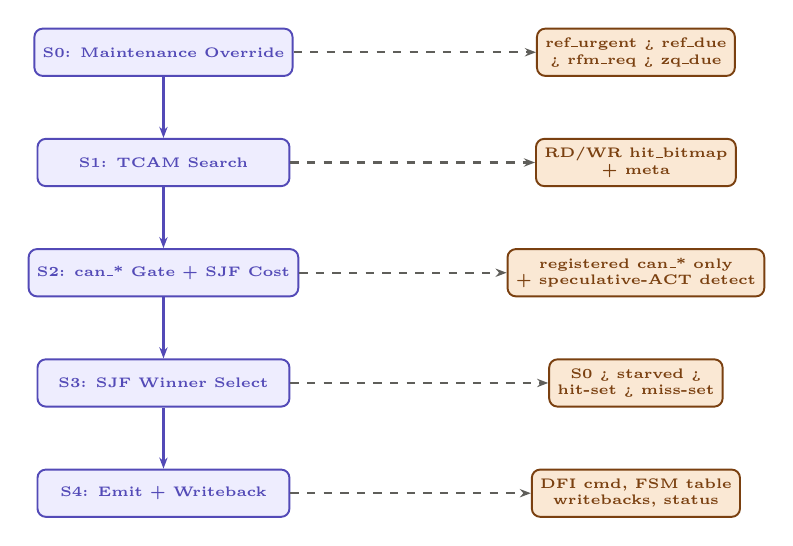
\begin{tikzpicture}[x=1cm,y=1cm]
    \node[sblk=Purp/PurpF,minimum width=3.2cm] (s0) at (0,4)  {S0: Maintenance Override};
    \node[sblk=Purp/PurpF,minimum width=3.2cm] (s1) at (0,2.6){S1: TCAM Search};
    \node[sblk=Purp/PurpF,minimum width=3.2cm] (s2) at (0,1.2){S2: can\_* Gate + SJF Cost};
    \node[sblk=Purp/PurpF,minimum width=3.2cm] (s3) at (0,-0.2){S3: SJF Winner Select};
    \node[sblk=Purp/PurpF,minimum width=3.2cm] (s4) at (0,-1.6){S4: Emit + Writeback};
    \draw[arr=Purp](s0)--(s1); \draw[arr=Purp](s1)--(s2);
    \draw[arr=Purp](s2)--(s3); \draw[arr=Purp](s3)--(s4);

    \node[sblk=Amber/AmberF] (ovr) at (6,4)   {ref\_urgent > ref\_due\\> rfm\_req > zq\_due};
    \node[sblk=Amber/AmberF] (tcam) at (6,2.6){RD/WR hit\_bitmap\\+ meta};
    \node[sblk=Amber/AmberF] (gate) at (6,1.2){registered can\_* only\\+ speculative-ACT detect};
    \node[sblk=Amber/AmberF] (win) at (6,-0.2){S0 > starved >\\hit-set > miss-set};
    \node[sblk=Amber/AmberF] (emit) at (6,-1.6){DFI cmd, FSM table\\writebacks, status};
    \draw[arr=MGray,dashed](s0)--(ovr); \draw[arr=MGray,dashed](s1)--(tcam);
    \draw[arr=MGray,dashed](s2)--(gate); \draw[arr=MGray,dashed](s3)--(win);
    \draw[arr=MGray,dashed](s4)--(emit);
  \end{tikzpicture}}
  \end{center}
  \infocard{Purp}{PurpF}{%
    \scriptsize \textbf{NOP-cycle priority (when \texttt{winner\_valid==0}):}
    1) opportunity REFsb (correctness/spread first) \quad
    2) speculative prefetch ACT (TCAM-confirmed, zero mispredict path) \quad
    3) WR-partition drain \quad 4) true NOP.
    \textbf{Starvation} is staggered (\texttt{age >= THR + entry\_idx}) so at most one
    starved miss can fire per cycle — no collision between two "must-service" candidates.
  }
\end{frame}

% ── Slide 10: FSM Tables ──────────────────────────────────────────────────────
\begin{frame}{FSM Tables}
              {What Stage 4 writes and Stage 2 reads}
  \begin{columns}[T,totalwidth=\linewidth]
    \begin{column}{0.32\linewidth}
      \infocard{Green}{GreenF}{%
        {\small\bfseries\color{Green}Per-Bank}\\
        \scriptsize $16{\times}$N\_RANKS rows. 8-state bank FSM, open row,
        next\_\{cas,pre,act,ref\} + can\_* pairs. Old pending-bits removed —
        redundant once TCAM hit/state covers them.
      }
    \end{column}
    \begin{column}{0.32\linewidth}
      \infocard{Blue}{BlueF}{%
        {\small\bfseries\color{Blue}Per-Rank}\\
        \scriptsize N\_RANKS rows. Rank FSM, REFab/ZQcal/PDX/SRX deadlines,
        leaky-bucket refresh credits, per-bank RAA[16] for RFM, MR4 thermal
        poll state.
      }
    \end{column}
    \begin{column}{0.32\linewidth}
      \infocard{Amber}{AmberF}{%
        {\small\bfseries\color{Amber}Global Timing}\\
        \scriptsize 1 instance. Cross-bank tRRD\_S/tCCD\_S, tFAW ring buffer,
        per-bank-group tRRD\_L/tCCD\_L/tWTR\_L family.
      }
    \end{column}
  \end{columns}
  \vspace{6pt}
  \infocard{MGray}{LGray}{%
    {\small\bfseries\color{MGray}Bank Activity Counter — small table, heavily shared}\\[2pt]
    \scriptsize \texttt{count | dirty} per bank. ME targets least-loaded bank for
    opportunistic refresh; Power Mgmt uses \texttt{count==0} across all banks as its
    power-down gate; Scheduler Stage 3 prefers draining high-count banks first.
  }
\end{frame}

% ── Slide 11: Maintenance Engine ─────────────────────────────────────────────
\begin{frame}{Maintenance Engine — 6 Sub-FSMs}
              {A peer to the Scheduler; never issues a CAS itself}
  \begin{center}
  \scalebox{0.68}{%
  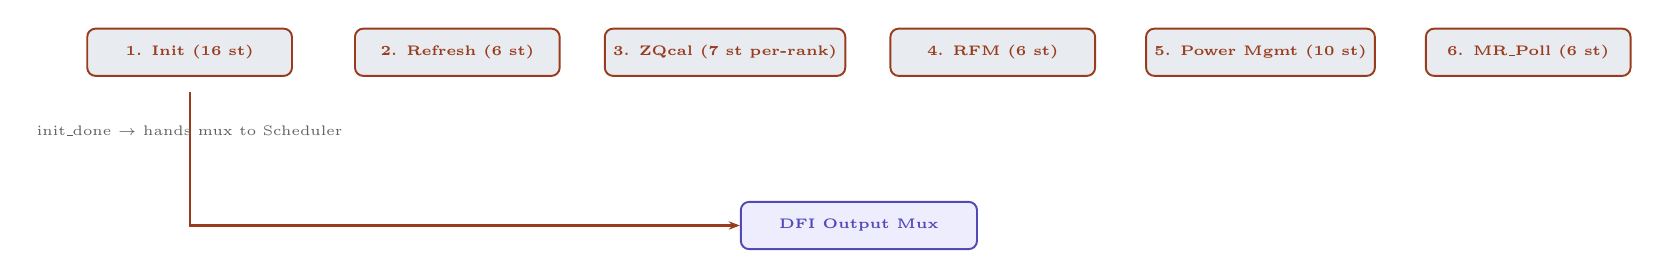
\begin{tikzpicture}[x=1cm,y=1cm]
    \foreach \n/\lbl/\x in {1/Init (16 st)/0, 2/Refresh (6 st)/3.4,
                            3/ZQcal (7 st per-rank)/6.8, 4/RFM (6 st)/10.2,
                            5/Power Mgmt (10 st)/13.6, 6/MR\_Poll (6 st)/17.0}{
      \node[sblk=BypassR/LGray,minimum width=2.6cm] at (\x,0) {\n. \lbl};
    }
    \node[sblk=Purp/PurpF,minimum width=3.0cm] (mux) at (8.5,-2.2) {DFI Output Mux};
    \draw[arr=BypassR] (0,-0.5) |- (mux.west);
    \node[font=\tiny,text=MGray] at (0,-1.0){init\_done $\to$ hands mux to Scheduler};
  \end{tikzpicture}}
  \end{center}
  \infocard{BypassR}{LGray}{%
    \scriptsize \textbf{Internal priority:} \texttt{ref\_urgent > ref\_due > rfm\_req >
    zq\_due} — mirrors Scheduler Stage 0 exactly. \textbf{Refresh FSM} runs a
    leaky-bucket credit counter, targets least-loaded bank for REFsb unless a
    per-bank watchdog (uncovered $>$ tREFI$\times$32) forces an overdue bank; fires free
    \emph{opportunity refresh} on true NOP cycles. \textbf{MR\_Poll} reads MR4 TUF —
    TUF=1 ($>$85\textdegree C) halves effective tREFI; response arrives via a
    \emph{sideband} from Read Data Path, not the response FIFO. \textbf{DFI mux}:
    \texttt{init\_done} is a one-way latch — Init FSM drives DFI until it fires, then
    Scheduler drives it forever after.
  }
\end{frame}

% ── Slide 12: Bank Partition + Speculative ACT ───────────────────────────────
\begin{frame}{Bank Partition \& Speculative Prefetch ACT}
              {Two techniques that hide latency for free}
  \infocard{Green}{GreenF}{%
    {\small\bfseries\color{Green}RD/WR Bank Partitioning}\\[2pt]
    \scriptsize Banks split into a read-half / write-half that rotate every
    \texttt{WINDOW\_SIZE} cycles. Read and write never share a bank inside a window,
    so \texttt{tRTW}/\texttt{tWTR} simply don't apply within it — the turnaround
    penalty is paid once, at the rotation boundary, amortized across the whole window.
  }
  \vspace{6pt}
  \infocard{Amber}{AmberF}{%
    {\small\bfseries\color{Amber}Speculative Prefetch ACT — NOP-cycle only, TCAM-confirmed}\\[2pt]
    \scriptsize Fires only when \texttt{winner\_valid==0} (a true NOP). If an active
    bank is approaching its column boundary
    (\texttt{COL\_MAX - cur\_col <= BL\_BYTES}), predict
    \texttt{\{same rank, same bg, bank+1, same row\}} — but only emit the ACT if
    RD\_TCAM confirms a real request already exists for that bank \emph{and} the row
    matches \emph{and} \texttt{bank\_act\_count > 0} \emph{and} \texttt{can\_act} +
    \texttt{can\_faw} both hold. No mispredict path exists — worst case is a wasted
    FAW slot if the row later conflicts, nothing worse.
  }
  \vspace{6pt}
  \infocard{MGray}{LGray}{%
    \scriptsize \texttt{bank\_act\_count} dual-use: \texttt{0} $\to$ no speculation,
    closed-page policy \textbullet\ \texttt{1--3} $\to$ speculate if boundary imminent,
    adaptive page \textbullet\ \texttt{$\geq$4} $\to$ speculate aggressively, open page.
    New hardware cost: one comparator per active bank + one mux — zero new tables,
    FSMs, or buffers.
  }
\end{frame}

% ── Slide 13: Sizing Rationale ────────────────────────────────────────────────
\begin{frame}{Why the Numbers Are What They Are}
              {A few constants worth remembering the reasoning for}
  \begin{center}
  \scriptsize
  \renewcommand{\arraystretch}{1.35}
  \begin{tabular}{p{3.6cm}p{2.4cm}p{7.2cm}}
    \toprule
    \textbf{\color{Blue}Parameter} & \textbf{\color{Blue}Value} & \textbf{\color{Blue}Why} \\
    \midrule
    N\_WR\_ENTRIES & 2--3$\times$ N\_RD & Writes drain in background; bigger WR buffer
      $\to$ lower RD latency at unchanged bandwidth \\
    GC\_WIDTH & 20b baseline & Half-range 524{,}288 cyc vs worst-case gap $\sim$12{,}480
      cyc $\to$ 42$\times$ margin (TCP-style wraparound compare) \\
    ROB\_WATERMARK & 37 cyc & Measured worst-case full round trip (row miss, no REF) \\
    REF-stall timeout & 76 cyc & 2$\times$ ROB watermark — "wait for in-flight CAS,"
      not abort-and-retry \\
    RD\_STARVATION\_THR & 12{,}480 cyc (9$\times$tREFI) & Read latency is user-visible;
      short leash \\
    WR\_STARVATION\_THR & 37{,}440 cyc (3$\times$RD) & Writes already drained
      preferentially — this is a backstop only \\
    FIFO\_DEPTH & 16 (both async FIFOs) & $\sim$2$\times$ CDC+pipeline round-trip latency \\
    TCAM budget & 38{,}784T $\approx$ 6{,}464 SRAM-bit eq. & RD\_TCAM (ternary,
      2-field) far cheaper than WR\_TCAM (exact, 4-field) — payoff of splitting by
      search semantics \\
    \bottomrule
  \end{tabular}
  \end{center}
\end{frame}

% ── Slide 14: Core Rules ──────────────────────────────────────────────────────
\begin{frame}{The Four Core Rules}
              {What every decision above ultimately answers to}
  \infocard{Purp}{PurpF}{%
    {\small\bfseries\color{Purp}R1 — The Scheduler never writes state directly}\\[2pt]
    \scriptsize Only through Stage 4's committed writebacks. Stages 0--3 are pure
    decision logic — nothing they compute is visible anywhere else until Stage 4
    commits it.
  }
  \vspace{5pt}
  \infocard{Blue}{BlueF}{%
    {\small\bfseries\color{Blue}R2 — Every register has exactly one owner}\\[2pt]
    \scriptsize Status registers $\to$ watermark managers. FSM tables $\to$ Stage 4
    (+ ME for maintenance events). timing\_reg\_file $\to$ CSR. Scheduler's access to
    anything it doesn't own is READ ONLY, always.
  }
  \vspace{5pt}
  \infocard{Green}{GreenF}{%
    {\small\bfseries\color{Green}R3 — State changes only via a committed command}\\[2pt]
    \scriptsize No speculative state mutation anywhere — even speculative-ACT only
    fires once TCAM has confirmed the request it's speculating about actually exists.
  }
  \vspace{5pt}
  \infocard{Amber}{AmberF}{%
    {\small\bfseries\color{Amber}R4 — Everything else is read-only}\\[2pt]
    \scriptsize If a block isn't the documented owner of a piece of state, it reads
    it and nothing more.
  }
\end{frame}

% ── Slide 15: Rating + Roadmap ────────────────────────────────────────────────
\begin{frame}{Where This Stands}
              {Self-rating and what's left before RTL}
  \begin{columns}[T,totalwidth=\linewidth]
    \begin{column}{0.49\linewidth}
      \infocard{Teal}{TealF}{%
        {\small\bfseries\color{Teal}Architecture Rating (v1.9.2+, unchanged through v1.9.8)}\\[3pt]
        \scriptsize
        Buffers, timing model, RAW bypass, scheduler: \textbf{9/10}\\
        vs. industry practice: \textbf{8/10}\\
        vs. typical capstone: \textbf{significantly above}\\[3pt]
        \textit{TCAM split, registered can\_* flags, credit-based CDC, SJF scheduling,
        bank pipelining, staggered starvation all match or exceed patterns in real
        DDRC IP (Synopsys DDRC, ARM DMC-620 class).}
      }
    \end{column}
    \begin{column}{0.49\linewidth}
      \infocard{BypassR}{LGray}{%
        {\small\bfseries\color{BypassR}Before RTL (priority order)}\\[3pt]
        \scriptsize
        1. Patch stale LaTeX docs (BUG-02..07 — pending bits, hardcoded depths,
        RAW partial-hit description)\\
        2. OQ-19b — channel-interleave granularity via Python traffic-trace script\\
        3. RTL skeleton — top-level hierarchy, parameter propagation\\[3pt]
        \textit{Only open architectural question left: OQ-19b. Everything else in the
        v1.0.1--v1.9.8 history is closed.}
      }
    \end{column}
  \end{columns}
\end{frame}

\end{document}
